% Figure 1: mo:os Kernel Architecture — Layered Separation
% Pure core (no IO) → Effect shell (RWMutex) → HTTP transport
\begin{figure}[t]
\centering
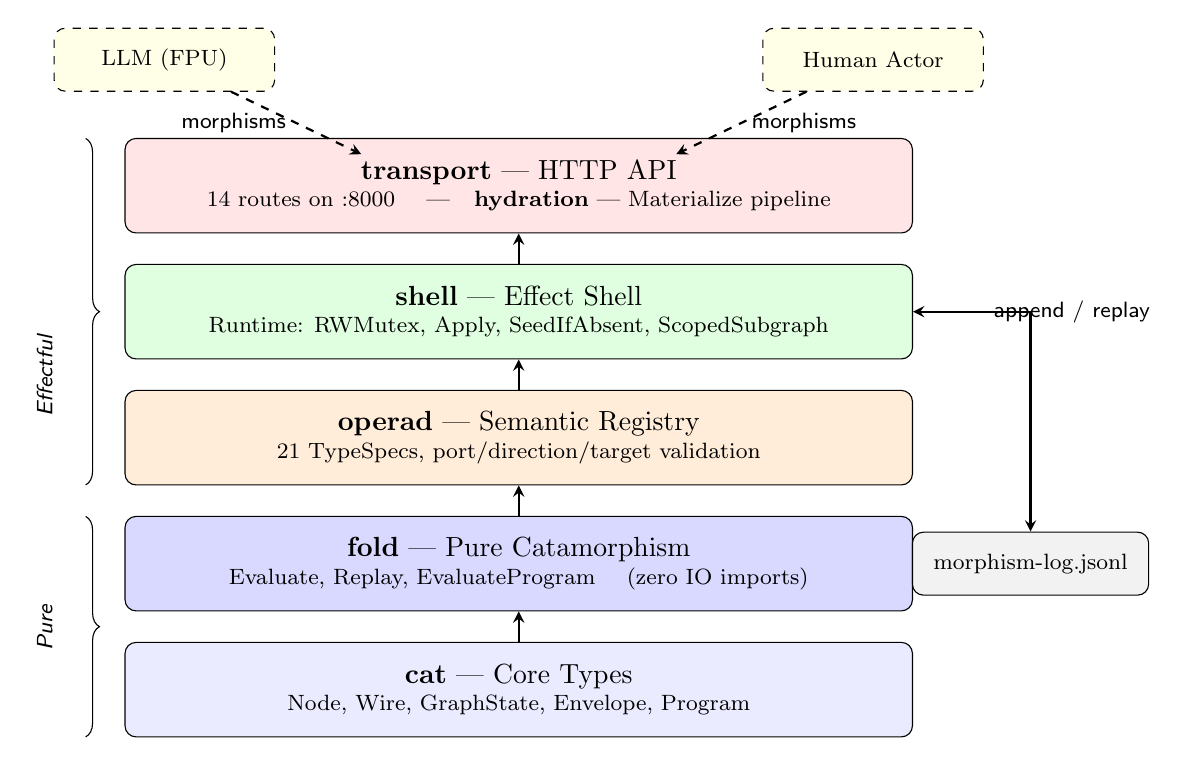
\begin{tikzpicture}[
  layer/.style={draw, rounded corners, minimum width=10cm, minimum height=1.2cm, align=center},
  arrow/.style={->, thick, >=stealth},
  label/.style={font=\footnotesize\sffamily}
]

% Layers (bottom to top)
\node[layer, fill=blue!8] (types) at (0,0) {\textbf{cat} — Core Types\\[-2pt]
  \footnotesize Node, Wire, GraphState, Envelope, Program};

\node[layer, fill=blue!15] (fold) at (0,1.6) {\textbf{fold} — Pure Catamorphism\\[-2pt]
  \footnotesize Evaluate, Replay, EvaluateProgram \quad (zero IO imports)};

\node[layer, fill=orange!15] (operad) at (0,3.2) {\textbf{operad} — Semantic Registry\\[-2pt]
  \footnotesize 21 TypeSpecs, port/direction/target validation};

\node[layer, fill=green!12] (shell) at (0,4.8) {\textbf{shell} — Effect Shell\\[-2pt]
  \footnotesize Runtime: RWMutex, Apply, SeedIfAbsent, ScopedSubgraph};

\node[layer, fill=red!10] (transport) at (0,6.4) {\textbf{transport} — HTTP API\\[-2pt]
  \footnotesize 14 routes on :8000 \quad|\quad \textbf{hydration} — Materialize pipeline};

% Arrows
\draw[arrow] (types) -- (fold);
\draw[arrow] (fold) -- (operad);
\draw[arrow] (operad) -- (shell);
\draw[arrow] (shell) -- (transport);

% Side labels
\node[label, rotate=90, anchor=south] at (-5.8,0.8) {\textit{Pure}};
\node[label, rotate=90, anchor=south] at (-5.8,4.0) {\textit{Effectful}};

% Brace for pure section
\draw[decorate, decoration={brace, amplitude=5pt, mirror}] (-5.5,-0.6) -- (-5.5,2.2);
\draw[decorate, decoration={brace, amplitude=5pt, mirror}] (-5.5,2.6) -- (-5.5,7.0);

% External actors
\node[draw, dashed, rounded corners, minimum width=2.8cm, minimum height=0.8cm, fill=yellow!10] (llm) at (-4.5,8.0) {\footnotesize LLM (FPU)};
\node[draw, dashed, rounded corners, minimum width=2.8cm, minimum height=0.8cm, fill=yellow!10] (human) at (4.5,8.0) {\footnotesize Human Actor};

\draw[arrow, dashed] (llm) -- node[left, label] {morphisms} (-2,6.8);
\draw[arrow, dashed] (human) -- node[right, label] {morphisms} (2,6.8);

% JSONL log
\node[draw, rounded corners, minimum width=3cm, minimum height=0.8cm, fill=gray!10] (log) at (6.5,1.6) {\footnotesize morphism-log.jsonl};
\draw[arrow, <->] (shell.east) -| node[right, label, pos=0.3] {append / replay} (log);

\end{tikzpicture}
\caption{Layered architecture of the \texttt{mo:os} kernel. The pure core
(\texttt{cat} + \texttt{fold}) contains zero IO imports. The effect shell
wraps it with \texttt{sync.RWMutex} for concurrent access. Both LLM agents
and human actors interact exclusively through typed morphism envelopes.}
\label{fig:architecture}
\end{figure}
